%% production_structure.tex
%% Nested CES production structure of DGE-METRIC.
%% Compile with: pdflatex production_structure.tex
\documentclass[tikz,border=14pt]{standalone}
\usepackage{tikz}
\usepackage{amsmath}
\usetikzlibrary{positioning,arrows.meta,calc,backgrounds,fit}

%% ---- colour palette (matches existing model diagrams) -----------------
\definecolor{Crimson}{RGB}{150,15,15}
\definecolor{CrimsonMid}{RGB}{175,45,45}
\definecolor{CrimsonLight}{RGB}{200,75,75}
\definecolor{CoalGray}{RGB}{75,75,90}
\definecolor{ForestGreen}{RGB}{25,115,65}
\definecolor{NavyBlue}{RGB}{25,60,130}
\definecolor{AmberOrange}{RGB}{195,100,15}

\begin{document}
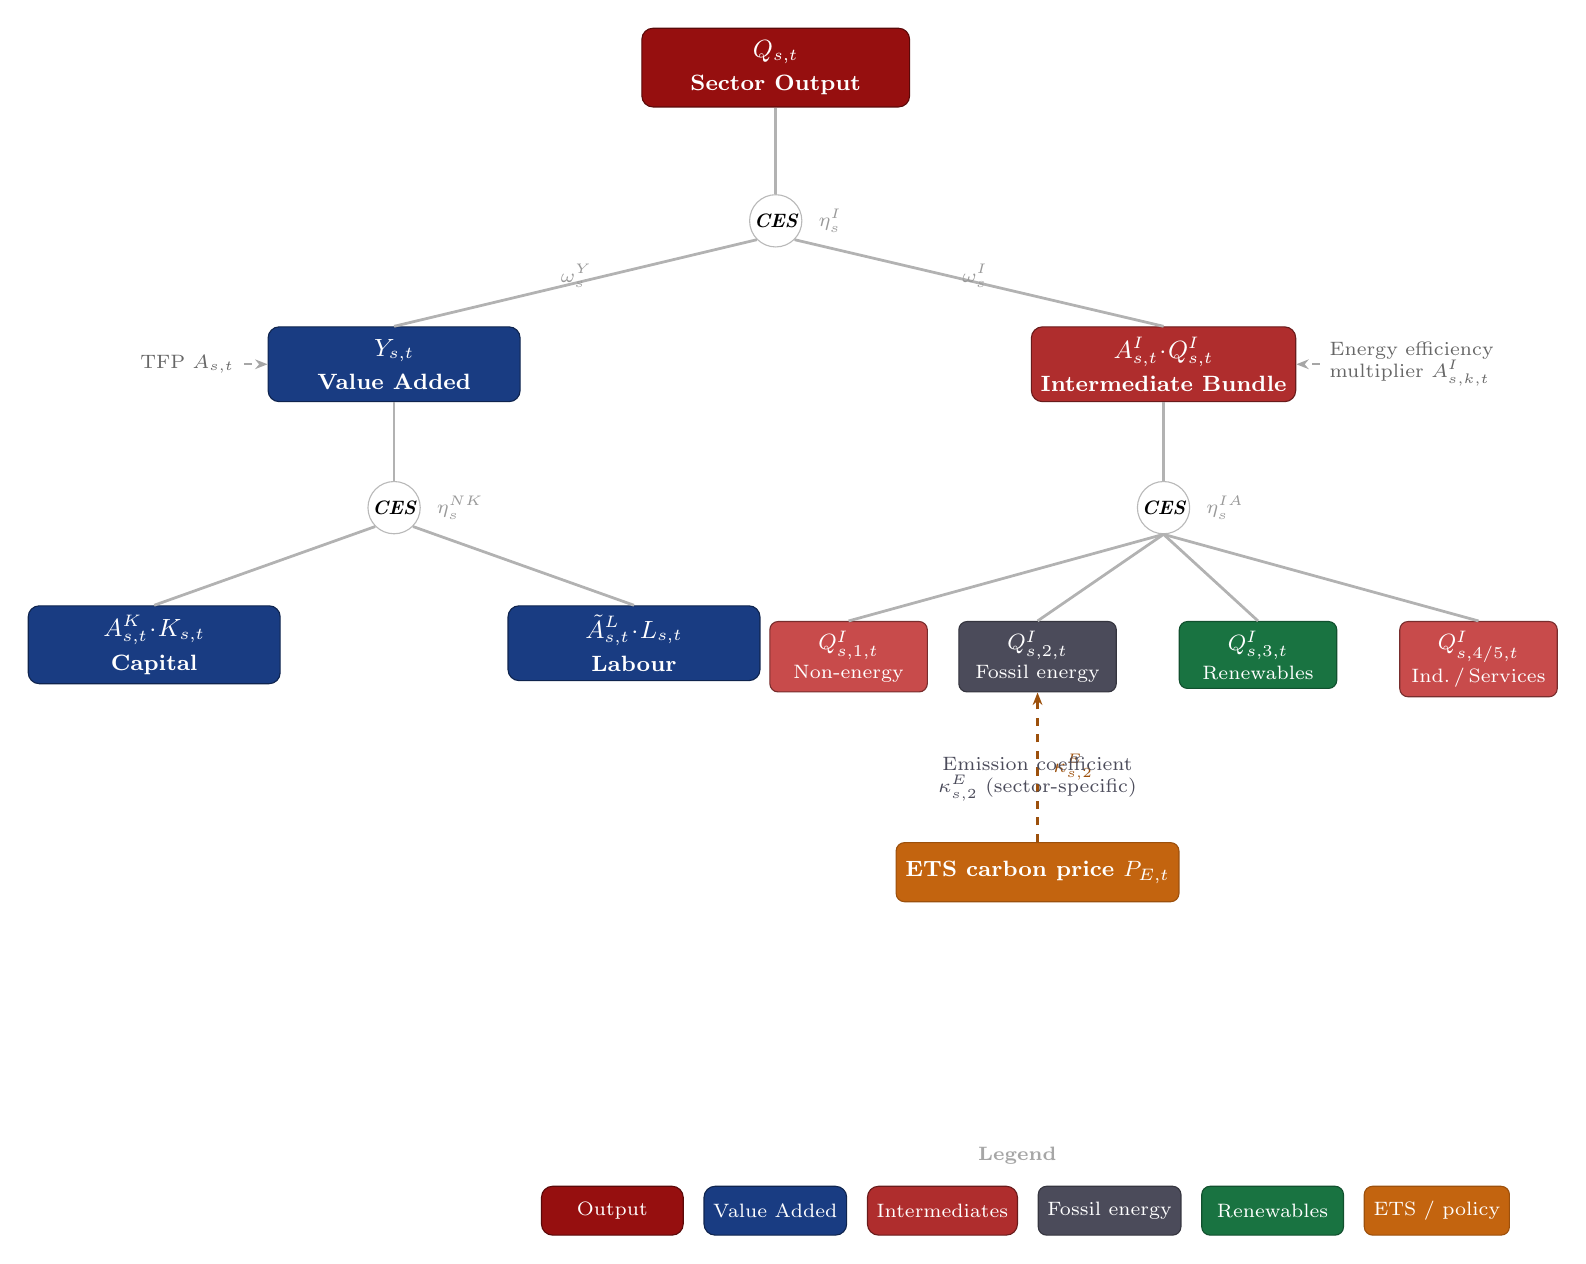
\begin{tikzpicture}[
  %% --- shared styles ----------------------------------------
  mainbox/.style={
    rectangle, rounded corners=4pt,
    fill=Crimson, draw=Crimson!60!black,
    text=white, font=\bfseries\small,
    minimum width=3.4cm, minimum height=1.0cm, align=center
  },
  vabox/.style={
    rectangle, rounded corners=4pt,
    fill=NavyBlue, draw=NavyBlue!60!black,
    text=white, font=\bfseries\small,
    minimum width=3.2cm, minimum height=0.95cm, align=center
  },
  intbox/.style={
    rectangle, rounded corners=4pt,
    fill=CrimsonMid, draw=CrimsonMid!60!black,
    text=white, font=\bfseries\small,
    minimum width=3.2cm, minimum height=0.95cm, align=center
  },
  leafbox/.style={
    rectangle, rounded corners=3pt,
    fill=CrimsonLight, draw=CrimsonLight!60!black,
    text=white, font=\footnotesize,
    minimum width=2.0cm, minimum height=0.85cm, align=center
  },
  fossilbox/.style={
    rectangle, rounded corners=3pt,
    fill=CoalGray, draw=CoalGray!70!black,
    text=white, font=\footnotesize,
    minimum width=2.0cm, minimum height=0.85cm, align=center
  },
  renewbox/.style={
    rectangle, rounded corners=3pt,
    fill=ForestGreen, draw=ForestGreen!70!black,
    text=white, font=\footnotesize,
    minimum width=2.0cm, minimum height=0.85cm, align=center
  },
  etsbox/.style={
    rectangle, rounded corners=3pt,
    fill=AmberOrange, draw=AmberOrange!80!black,
    text=white, font=\footnotesize\bfseries,
    minimum width=2.6cm, minimum height=0.75cm, align=center
  },
  cescirc/.style={
    circle, fill=white, draw=gray!55,
    font=\scriptsize\itshape\bfseries,
    minimum size=0.62cm, inner sep=1pt
  },
  branch/.style={line width=1.0pt, gray!60},
  annotarr/.style={
    -{Stealth[length=4.5pt,width=3.5pt]},
    line width=0.8pt, dashed
  },
]

%% ============================================================
%% ROW 0 — sector output
%% ============================================================
\node[mainbox] (Q) at (0,0) {$Q_{s,t}$\\[1pt]\footnotesize Sector Output};

%% CES nest 1 (between Q and its children)
\node[cescirc, below=1.1cm of Q] (ces1) {CES};
\draw[branch] (Q.south) -- (ces1.north);

%% label the elasticity
\node[right=0.08cm of ces1, font=\scriptsize, text=gray!80] {$\eta^{I}_{s}$};

%% ============================================================
%% ROW 1 — value added  |  intermediate bundle
%% ============================================================
\node[vabox,  below left  = 1.1cm and 3.0cm of ces1] (Y)  {$Y_{s,t}$\\[1pt]\footnotesize Value Added};
\node[intbox, below right = 1.1cm and 3.0cm of ces1] (QI) {$A^{I}_{s,t}\!\cdot\!Q^{I}_{s,t}$\\[1pt]\footnotesize Intermediate Bundle};

\draw[branch] (ces1.south west) -- (Y.north);
\draw[branch] (ces1.south east) -- (QI.north);

%% share labels on branches
\node at ($(ces1.south west)!0.42!(Y.north)$) [left=1pt, font=\scriptsize, text=gray!80] {$\omega^{Y}_{s}$};
\node at ($(ces1.south east)!0.42!(QI.north)$) [right=1pt, font=\scriptsize, text=gray!80] {$\omega^{I}_{s}$};

%% EE shock annotation on intermediate bundle
\node[right=0.30cm of QI, align=left, font=\scriptsize, text=gray!80!black] (eeann)
  {Energy efficiency\\multiplier $A^{I}_{s,k,t}$};
\draw[annotarr, gray!70] (eeann.west) -- (QI.east);

%% TFP annotation on value added
\node[left=0.30cm of Y, align=right, font=\scriptsize, text=gray!80!black] (tfpann)
  {TFP $A_{s,t}$};
\draw[annotarr, gray!70] (tfpann.east) -- (Y.west);

%% CES nests below Y and QI
\node[cescirc, below=1.0cm of Y]  (ces2) {CES};
\node[cescirc, below=1.0cm of QI] (ces3) {CES};
\draw[branch] (Y.south)  -- (ces2.north);
\draw[branch] (QI.south) -- (ces3.north);
\node[right=0.08cm of ces2, font=\scriptsize, text=gray!80] {$\eta^{NK}_{s}$};
\node[right=0.08cm of ces3, font=\scriptsize, text=gray!80] {$\eta^{IA}_{s}$};

%% ============================================================
%% ROW 2 — capital & labour  |  five sectoral intermediates
%% ============================================================

%% --- Capital & Labour ---
\node[vabox, below left  = 1.0cm and 1.2cm of ces2] (K)
  {$A^{K}_{s,t}\!\cdot\! K_{s,t}$\\[1pt]\footnotesize Capital};
\node[vabox, below right = 1.0cm and 1.2cm of ces2] (L)
  {$\tilde{A}^{L}_{s,t}\!\cdot\! L_{s,t}$\\[1pt]\footnotesize Labour};

\draw[branch] (ces2.south west) -- (K.north);
\draw[branch] (ces2.south east) -- (L.north);

%% --- Five sectoral intermediate inputs (centred under ces3) ---
\coordinate (cesbot) at (ces3.south);

\node[leafbox,   below=1.1cm of ces3, xshift=-4.0cm] (QI1)
  {$Q^{I}_{s,1,t}$\\[1pt]\scriptsize Non-energy};
\node[fossilbox, below=1.1cm of ces3, xshift=-1.6cm] (QI2)
  {$Q^{I}_{s,2,t}$\\[1pt]\scriptsize Fossil energy};
\node[renewbox,  below=1.1cm of ces3, xshift=+1.2cm] (QI3)
  {$Q^{I}_{s,3,t}$\\[1pt]\scriptsize Renewables};
\node[leafbox,   below=1.1cm of ces3, xshift=+4.0cm] (QI45)
  {$Q^{I}_{s,4/5,t}$\\[1pt]\scriptsize Ind.\,/\,Services};

%% branches from ces3 to each intermediate
\foreach \nd in {QI1,QI2,QI3,QI45}{
  \draw[branch] (cesbot) -- (\nd.north);
}

%% ============================================================
%% ETS / carbon price annotation
%% ============================================================
\node[etsbox, below=1.9cm of QI2] (ets)
  {ETS carbon price $P_{E,t}$};

\draw[annotarr, AmberOrange!80!black, line width=1pt]
  (ets.north) -- (QI2.south)
  node[midway, right=2pt, font=\scriptsize, text=AmberOrange!80!black]
  {$\kappa^{E}_{s,2}$};

%% ============================================================
%% Emission intensity footnote under fossil box
%% ============================================================
\node[below=0.15cm of QI2, font=\scriptsize, text=CoalGray,
      align=center, yshift=-0.55cm]
  {Emission coefficient\\$\kappa^{E}_{s,2}$ (sector-specific)};


%% ============================================================
%% Legend — horizontal row centred below the full diagram
%% ============================================================
\node[mainbox,   minimum width=1.8cm, minimum height=0.62cm,
      font=\scriptsize, below=3.6cm of ets, xshift=-5.4cm] (l1) {Output};
\node[vabox,     minimum width=1.8cm, minimum height=0.62cm,
      font=\scriptsize, right=0.25cm of l1] (l2) {Value Added};
\node[intbox,    minimum width=1.8cm, minimum height=0.62cm,
      font=\scriptsize, right=0.25cm of l2] (l3) {Intermediates};
\node[fossilbox, minimum width=1.8cm, minimum height=0.62cm,
      font=\scriptsize, right=0.25cm of l3] (l4) {Fossil energy};
\node[renewbox,  minimum width=1.8cm, minimum height=0.62cm,
      font=\scriptsize, right=0.25cm of l4] (l5) {Renewables};
\node[etsbox,    minimum width=1.8cm, minimum height=0.62cm,
      font=\scriptsize, right=0.25cm of l5] (l6) {ETS / policy};
\node[above=0.15cm of l3, xshift=0.95cm,
      font=\scriptsize\bfseries, text=gray!70] {Legend};

\end{tikzpicture}
\end{document}
